\documentclass{exercices}
\usepackage{ae, aeguill, graphicx}
\usepackage{fullpage}
\usepackage{xspace}
\usepackage{color}
\usepackage{amsmath, amssymb}
\usepackage{latexsym}
\usepackage{url}
\usepackage{tikz}
\usetikzlibrary{decorations}
\usetikzlibrary{decorations.fractals}

\usepackage{verbatim}

\renewcommand{\|}{\url|}
\begin{document}

\sujet{Java lab 1 - 17 october 2008}

The answers to the exercices below are due before \emph{20 October 2008}. 
The procedure to send the exercices is:
\begin{enumerate}
  \item Create a directory named \verb!yourname-lab1!.
  \item Copy all the \verb!.java! source files to this directory.
  \item Issue following command in a shell : \verb!tar czvf yourname-lab1.tar.gz yourname-lab1/!
        to create a tarball.
  \item Send this tarball to \verb!pablo@sifflez.org! with subject \verb!yourname-lab1!.
\end{enumerate}

\section{Java toolchain}
You will put each java class you write in its own file.

For a class named 'Example' you will use file \verb!example.java!.
To compile this class to bytecode you will execute:
\begin{verbatim}
  $ javac example.java
\end{verbatim}
If no errors are found this will produce a bytecode file named \verb!Example.class!.

To run a class that contains a \verb!main! method you will issue below command
in the directory containing \verb!Example.class!:
\begin{verbatim}
  $ java Example
\end{verbatim}

\section{Prime Numbers}
\begin{exercice}[\textbf{Numbers}]\\ 
Write a class \verb!Numbers! with a main method that prints the numbers from 1 to 100.
\end{exercice}
\begin{exercice}[\textbf{Primes - Naïve}]
\begin{enumerate}
\item
A naïve method for determining if a number $n$ is prime is checking that all the numbers smaller
than $\sqrt{n}$ are not divisors of $n$.

Add a static method "\verb!bool isPrime(long n)!" that implements this algorithm in the class \verb!Numbers!.
You might need to use the method \verb!double Math.sqrt(double n)!.
\item
 Modify \verb!Numbers! so that it prints all prime numbers smaller than 100.
\end{enumerate}
\end{exercice}

\begin{exercice}[\textbf{Eratosthenes sieve}]\\
Eratosthenes was a greek mathematician, geographer and astronomer which calculated using the
elevation of the sun what we believe to be the first measure of the earth circumference.
He also produced an efficient method to compute prime numbers smaller than $N$, which we
explain below.
\begin{center}
\framebox[0.75\textwidth][s]{
\begin{minipage}{0.6\textwidth}
\textbf{Eratosthenes algorithm:}
\hfill
\begin{enumerate}
\item Make a list of numbers from 2 to $N$, call it numbers.
\item Take an empty list and call it primes.
\item Take the smaller number $k$ in list numbers.
\item If $k$ is bigger than the square root of $\sqrt{N}$, stop.
\item Append $k$ to list primes.
\item Remove all the multiples of $k$ from numbers.
\item Start again at 3.
\end{enumerate}
\hfill
\end{minipage}
}
\end{center}

Implement this algorithm in java using arrays for the lists. Here are some guidelines to
help you, they are not mandatory:
\begin{itemize}
\item Create two arrays:
\begin{itemize}
\item \verb!numbers! of size \verb!N-1! and with \verb!bool! type
\item \verb!primes! of size bigger than $\sqrt{N}$ and with \verb!long! type.
\end{itemize}
\item \verb!numbers! is a bool array, it allows us to handle the list of numbers:
\begin{itemize}
\item if cell \verb!k! is \verb!true! that means that \verb!k! is still in list numbers
\item if cell \verb!k! is \verb!false! that means that \verb!k! has been removed from list numbers
\end{itemize}
\item \verb!primes! is used to store the primes when we find them.
\end{itemize}
\end{exercice}

\section{Turtle graphics}
In 1967 W. Feurzeig and S. Papert created a programming language called \emph{Logo} to teach programming.
This language allowed to move a turtle on a graphical screen to produce all kind of pictures.

You are going to use a java package called \verb!TurtleGraphics! to make some pictures using java.
The package \verb!TurtleGraphics! contains two classes:
\begin{itemize}
  \item \verb!class Sheet! \\
  The class Sheet implements a graphical window that we can draw onto.
  It provides the following methods:
  \begin{itemize}
    \item \verb!Sheet(int width, int height)!, the constructor, you must provide the dimensions of the graphical window.
  \end{itemize}
  \item \verb!class Turtle! \\
  \begin{itemize}
    \item \verb!public Turtle(Sheet sheet)!, the constructor, you must provide a sheet for the turtle to draw on.
    \item \verb!void turn(double degrees)!, makes the turtle turn.
    \item \verb!void advance(double steps)!, makes the turtle advance.
    \item \verb!void penDown()! and \verb!void penUp()!, change the pen state, when you move the turtle and the pen is down it will leave a trail on the sheet.
    \item \verb!void setPenColor(Color color)!, changes the pen color.
  \end{itemize}
\end{itemize}

For example the following program draws a Triangle:
\begin{verbatim}
import java.awt.Color;
import TurtleGraphics.Sheet;
import TurtleGraphics.Turtle;

public class AdvancedTurtle extends Turtle {
  public AdvancedTurtle(Sheet s) {
    super(s);
  }

  public void triangle(double side) {
    advance(side);
    turn(120);
    advance(side);
    turn(120);
    advance(side);
  }

  static public void main(String args[]) {
    Sheet sheet = new Sheet(300,300);
    AdvancedTurtle t = new AdvancedTurtle(sheet);
    t.penDown();
    t.triangle(50);
  }
}
\end{verbatim}


\begin{exercice}
  Add a method \verb!square! to AdvancedTurtle that draws a square of given side.
\end{exercice}

\begin{exercice}
  Add a method \verb!circle! that draws a circle of given radius.
\end{exercice}

\begin{exercice}[Koch's Snow Flake] \\
On 1904 Helge Von Koch described the fractal curve obtained by the following algorithm:

\begin{center}
\framebox[0.75\textwidth][s]{
\begin{minipage}{0.6\textwidth}
\textbf{Koch's algorithm:}
\hfill
\begin{enumerate}
\item take a segment. \\
\begin{tikzpicture}[decoration=Koch snowflake]
    \draw (0,0) -- (3,0) ;
\end{tikzpicture}

\item divide it in 4 new segments of \emph{equal length} according to the following picture:\\
\begin{tikzpicture}[decoration=Koch snowflake]
    \draw decorate{ (0,0) -- (3,0) };
\end{tikzpicture}
\item iterate this procedure for each new segment:\\
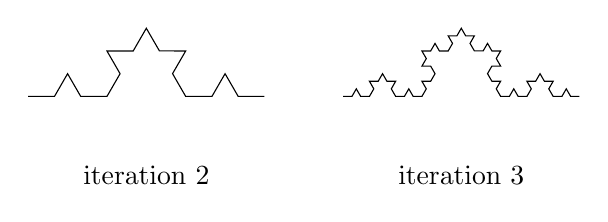
\begin{tikzpicture}[decoration=Koch snowflake]
    \draw decorate{ decorate{(0,0) -- (3,0) }};
    \node at(1.5,-1) {iteration 2};
    \draw decorate{ decorate{ decorate{ (4,0) -- (7,0) }}};
    \node at(5.5,-1) {iteration 3};
    \end{tikzpicture}
\end{enumerate}
\hfill
\end{minipage}
}
\begin{enumerate}
\item Add a method \verb!koch(double length)! that draws a Koch's curve of given length. 
\item Add a method \verb!snowFlake(double length)! that draws a Koch's snowflake, obtained
      by applying the Koch's algorithm to the three sides of an equilateral triangle:

\begin{center}
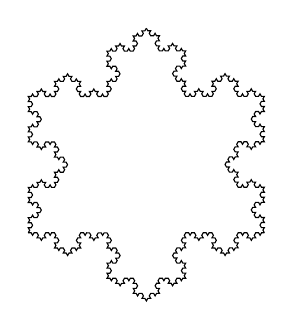
\begin{tikzpicture}[decoration=Koch snowflake]
    \draw decorate{ decorate{ decorate{ decorate{ (3,0) -- (0,0) }}}};
    \draw decorate{ decorate{ decorate{ decorate{ (0,0) -- (1.5,2.598) }}}};
    \draw decorate{ decorate{ decorate{ decorate{ (1.5,2.598) -- (3,0)}}}};
\end{tikzpicture}
\end{center}
\end{enumerate}
\end{center}
\end{exercice}

\end{document}
